\documentclass[11pt,a4paper]{article}

\usepackage[utf8]{inputenc}
\usepackage[T1]{fontenc}
\usepackage[english]{babel}
\usepackage{geometry}
\geometry{top=2.5cm, bottom=2.5cm, left=2.5cm, right=2.5cm}
\usepackage{fancyhdr}
\usepackage{lastpage}
\usepackage{booktabs}
\usepackage{tabularx}
\usepackage{longtable}
\usepackage{float}
\usepackage{graphicx}
\usepackage{xcolor}
\usepackage{hyperref}
\usepackage{listings}
\usepackage{enumitem}
\usepackage{amsmath,amssymb}
\usepackage{microtype}

\definecolor{navyblue}{RGB}{20, 50, 90}
\definecolor{codebg}{RGB}{248, 249, 250}

\hypersetup{
    colorlinks=true,
    linkcolor=navyblue,
    urlcolor=navyblue,
    citecolor=navyblue
}

\pagestyle{fancy}
\fancyhf{}
\fancyhead[L]{\small WellProdSim / EthosTerra}
\fancyhead[R]{\small Progress Report -- Week 9 (Block B6)}
\fancyfoot[C]{\small \thepage\ of \pageref{LastPage}}
\renewcommand{\headrulewidth}{0.4pt}
\renewcommand{\footrulewidth}{0pt}

\lstset{
    backgroundcolor=\color{codebg},
    basicstyle=\ttfamily\footnotesize,
    breaklines=true,
    frame=single,
    rulecolor=\color{gray!30},
    numbers=none,
    showstringspaces=false
}

\begin{document}

% ==============================================================================
% TITLE PAGE
% ==============================================================================
\begin{titlepage}
    \thispagestyle{empty}
    \centering
    \vspace*{1.5cm}

    {\large Universidad Tecnológica de Bolívar\par}
    \vspace{0.3cm}
    {\normalsize Master of Science in Engineering -- Research Seminar II\par}

    \vspace{2.2cm}
    {\LARGE\bfseries Territorial eBDI Atlas, Document Quarantine, and Epistemic Extraction with Local Micro-LLM\par}

    \vspace{0.8cm}
    {\large\itshape Progress Report -- Week 9 (Block B6)\par}

    \vspace{2.5cm}
    \begin{tabular}{ll}
        \textbf{Researcher:} & Jesús Martínez Velandia \\
        \textbf{Advisor:} & Jairo Serrano \\
        \textbf{Co-advisors:} & Edwin Puertas, Juan Martínez \\
        \textbf{Period:} & Week 9 of 16 \\
        \textbf{Block:} & B6 (Agrarian Corpus and Territorial Atlas) \\
        \textbf{Date:} & October 8, 2026 \\
    \end{tabular}

    \vfill
    {\small Consolidated technical release\par}
    \vspace*{1.0cm}
\end{titlepage}

\newpage
\pagenumbering{roman}
\fancyfoot[C]{\small \thepage}
\tableofcontents
\newpage

% ==============================================================================
% 1. SCOPE AND ROADMAP
% ==============================================================================
\pagenumbering{arabic}
\setcounter{page}{1}
\fancyfoot[C]{\small \thepage\ of \pageref{LastPage}}

\section{Scope of Week 9 in the Work Plan}

The sixteen-week master's thesis schedule positions Week 9 within Block B6, dedicated to populating agent beliefs with empirical documentary and geographical sources. Prior phases established the baseline intent classifier (Week 5), the Pure Case (Week 6), eBDI intent conflict resolution (Week 7), and decoupled manual intent management (Week 8). Block B6 grounds agent mental models in municipal empirical metrics and verified policy documents.

\begin{table}[H]
\centering
\small
\caption{Thesis progression by development blocks.}
\label{tab:schedule}
\begin{tabularx}{\textwidth}{lp{3.4cm}p{5.0cm}X}
\toprule
\textbf{Week} & \textbf{Block} & \textbf{Core Objective} & \textbf{Status} \\
\midrule
Week 5 & B1 (Baseline) & Base classifier evaluated on 20 synthetic cases & Completed (\texttt{388553e}) \\
Week 6 & B2--B3 (Pure Case) & Delimiters and Pydantic V2 contracts & Completed (\texttt{30090dc}) \\
Week 7 & B4 (Conflict Case) & Collision detection across 30 test cases & Completed (\texttt{b3f810a}) \\
Week 8 & B5 (Manual CRUD) & Decoupled storage and 30-day soft purge & Completed (\texttt{a140f22}) \\
\textbf{Week 9} & \textbf{B6 (Atlas \& Corpus)} & \textbf{Atlas AT-1, Quarantine, Gemma 4 \& YAML} & \textbf{Completed (\texttt{d17e44b})} \\
Weeks 10--12 & B7--B9 (Simulation) & Live multi-agent BDI cycle integration (BESA) & Scheduled \\
\bottomrule
\end{tabularx}
\end{table}

Key deliverables completed during this increment include:
\begin{itemize}[leftmargin=*]
    \item The AT-1 geospatial console covering the 15 PDET municipalities of Montes de María.
    \item The document quarantine subsystem enforcing SHA-256 integrity and human approval gates.
    \item The epistemic belief extraction pipeline running Gemma 4 over official regulatory texts.
    \item Deterministic compilation to executable YAML specifications (\texttt{GoalSpec} and \texttt{PlanSpec}).
    \item An adaptive document discovery protocol constrained to a strict maximum of six retries.
\end{itemize}

% ==============================================================================
% 2. LOCAL INFERENCE CONFIGURATION
% ==============================================================================
\section{Local Inference Configuration: Gemma 4}

To preserve data sovereignty and reproducible execution, all neural model inference runs strictly locally via Docker Model Runner (DMR) with zero external network calls:

\begin{itemize}[leftmargin=*]
    \item \textbf{Base model:} \texttt{ai/gemma4:E4B}, from Google DeepMind's Gemma 4 family, structured around 4 billion parameters (4B).
    \item \textbf{Quantization:} Post-training 4-bit integer quantization using the \texttt{MOSTLY\_Q4\_K\_M} GGUF profile.
    \item \textbf{Memory footprint:} 3.2\,GB of unified RAM on an Apple Silicon M4 chip (16\,GB host memory).
    \item \textbf{Execution latency:} Measured average of 18,420\,ms per 1,800-token regulatory passage.
    \item \textbf{Architectural role:} The LLM operates solely as an extraction candidate generator; it holds zero autonomous authority to approve documents or write final production files to disk.
\end{itemize}

% ==============================================================================
% 3. DETERMINISTIC PIPELINE VALIDATIONS
% ==============================================================================
\section{Deterministic Pipeline Validations}

To guarantee system stability and prevent hallucinated assertions from reaching simulation agents, data moving through the pipeline is screened across six independent deterministic layers:

\subsection{1. Binary File Integrity and Quarantine Isolation}
\begin{itemize}[leftmargin=*]
    \item \textbf{Magic bytes verification:} Uploaded and downloaded files are inspected across their initial four raw bytes to confirm the \texttt{\%PDF-} signature, rejecting polyglots or disguised binaries.
    \item \textbf{SHA-256 cryptographic identity:} Every document is indexed by its immutable SHA-256 hash in \texttt{outputs/atlas/artifacts/\{sha256\}.pdf}, eliminating storage duplicates.
    \item \textbf{Anti-SSRF network isolation:} The acquisition engine performs local DNS pre-resolution and categorically denies requests targeting \texttt{localhost}, loopback addresses (\texttt{127.0.0.1}), private RFC 1918 subnets (\texttt{10.0.0.0/8}, \texttt{172.16.0.0/12}, \texttt{192.168.0.0/16}), or cloud metadata endpoints (\texttt{169.254.169.254}).
\end{itemize}

\subsection{2. Structural Schema Enforcement (Pydantic V2)}
All API endpoints and internal transformers enforce Pydantic V2 schemas configured with \texttt{model\_config = ConfigDict(extra="forbid")}. Any undeclared key generated by the model triggers immediate schema validation failure, discarding the payload prior to persistence.

\subsection{3. Verbatim Grounding and Hallucination Filter}
Every extracted belief proposal must supply an exact quotation (\texttt{verbatim\_quote}) from the source. The verification script checks for an exact substring match within the unparsed source text:
\begin{equation}
    \text{State} = \begin{cases}
        \texttt{verified\_verbatim}, & \text{if } \text{verbatim\_quote} \subseteq \text{SourceText} \\
        \texttt{hallucination\_rejected}, & \text{otherwise}
    \end{cases}
\end{equation}
If any token differs from the source text, the proposal is marked as rejected and excluded from agent belief sets.

\subsection{4. Syntactic Validation of Activation Rules (MVEL)}
Approved beliefs define trigger conditions for agent plans. The compiler validates MVEL syntax (e.g., \texttt{belief.get('credito') == false}) and checks variables against the simulator's controlled vocabulary prior to generating YAML specs.

\subsection{5. Input Delimitation against Prompt Injection}
Document chunks are framed inside explicit XML boundaries (\texttt{<document\_chunk>}). System prompts restrict model behavior to passive JSON extraction, while regex scanners screen for override directives.

\subsection{6. Adaptive Discovery and Anti-Redundancy Filter}
When a reviewer discards a proposed document candidate and inputs feedback notes:
\begin{itemize}[leftmargin=*]
    \item The search engine refines query terms and executes up to six total retries (\texttt{max\_retries = 6}).
    \item Canonical URL schemes and title similarity matrices prevent proposing previously evaluated or rejected sources.
\end{itemize}

% ==============================================================================
% 4. VISUAL SYSTEM EVIDENCE
% ==============================================================================
\section{Visual Evidence: User Interface Operation}

Figures~\ref{fig:ui_map}, \ref{fig:ui_quarantine}, and \ref{fig:ui_dilemmas} show direct captures of the live application running on local port 5173, illustrating the three primary functional panels delivered in Block B6.

\subsection{Geospatial Console and Municipal Characterization}
Figure~\ref{fig:ui_map} shows the AT-1 Atlas Console. It displays DANE MGN 2024 boundary vectors for the 15 PDET municipalities of Montes de María alongside agronomic telemetry (IDEAM rainfall, peasant crops, and credit restriction indicators).

\begin{figure}[H]
    \centering
    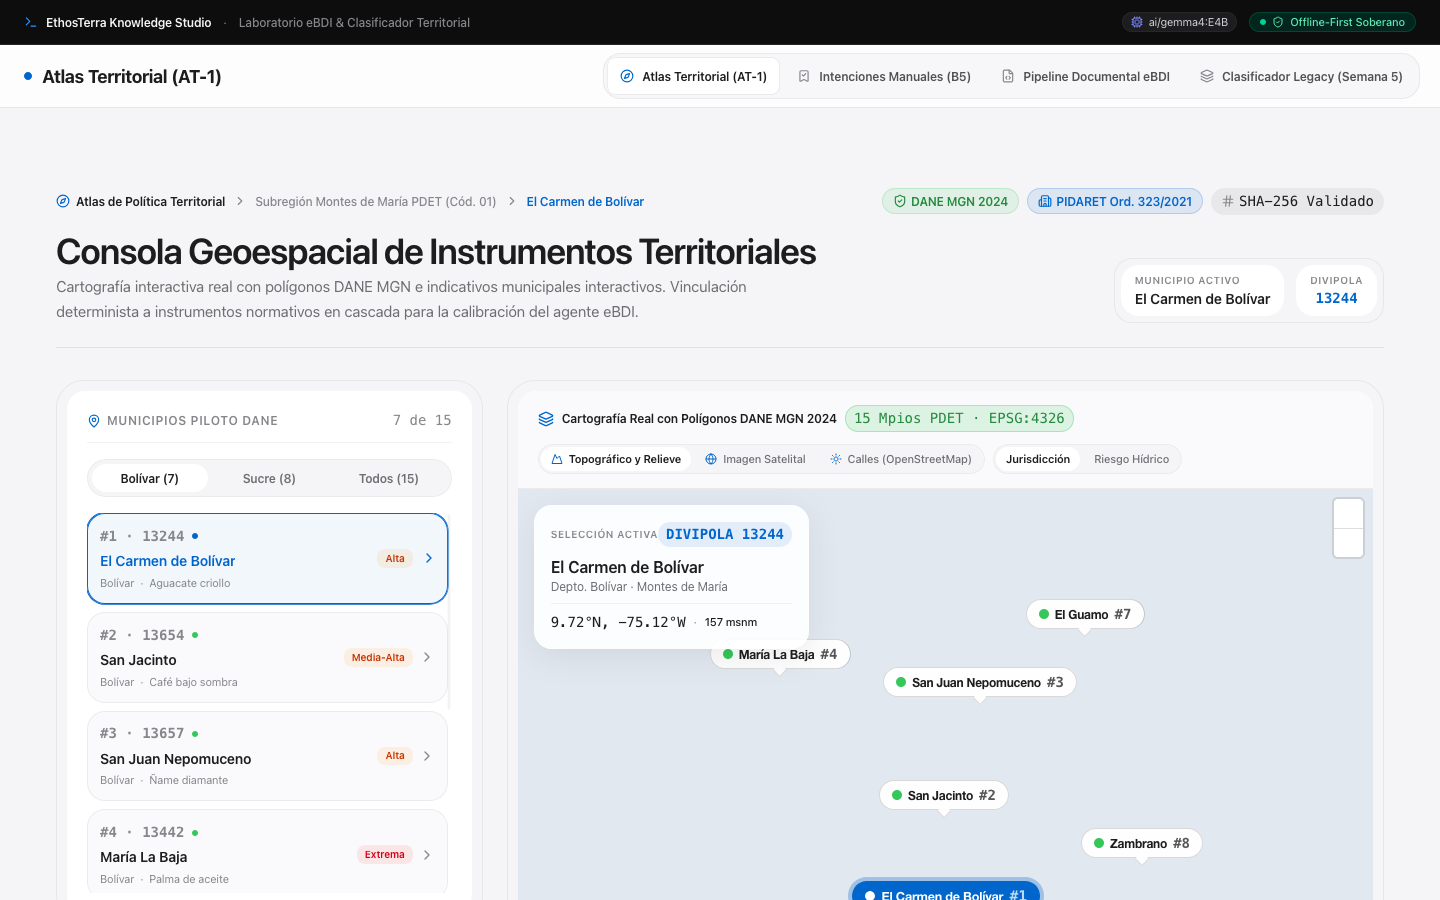
\includegraphics[width=0.96\textwidth]{docs/diagrams/out/ui_atlas_mapa_territorial.png}
    \caption{AT-1 Atlas Console: Montes de María territorial mapping and municipal agronomic profile.}
    \label{fig:ui_map}
\end{figure}

\subsection{Document Quarantine and Human Decision Gate}
Figure~\ref{fig:ui_quarantine} illustrates the quarantine candidate inspection view. For each candidate source, the UI exposes the agent's technical justification, the retry iteration badge, and human action buttons (\textit{Accept into Quarantine} or \textit{Discard with Feedback}).

\begin{figure}[H]
    \centering
    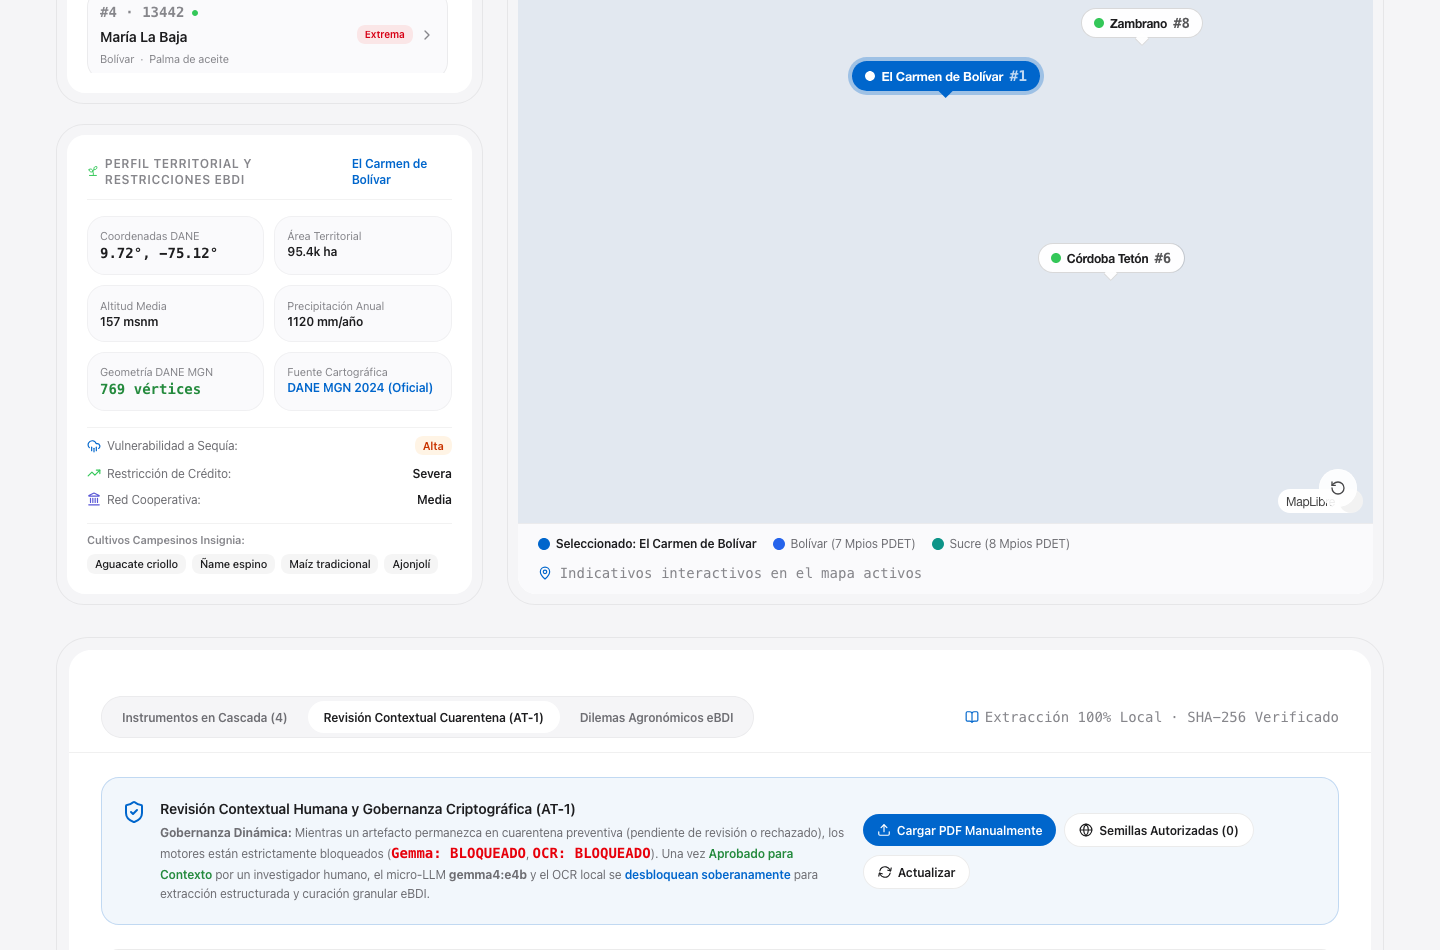
\includegraphics[width=0.96\textwidth]{docs/diagrams/out/ui_cuarentena_candidatos.png}
    \caption{Document Quarantine Panel: candidate discovery list, agent technical rationale, and human action gates.}
    \label{fig:ui_quarantine}
\end{figure}

\subsection{Agronomic Dilemmas Console and Compiled Beliefs}
Figure~\ref{fig:ui_dilemmas} presents extracted eBDI beliefs arranged by policy pillars (land tenure, water conservation, agrarian credit), displaying activation triggers and mapped plan operations.

\begin{figure}[H]
    \centering
    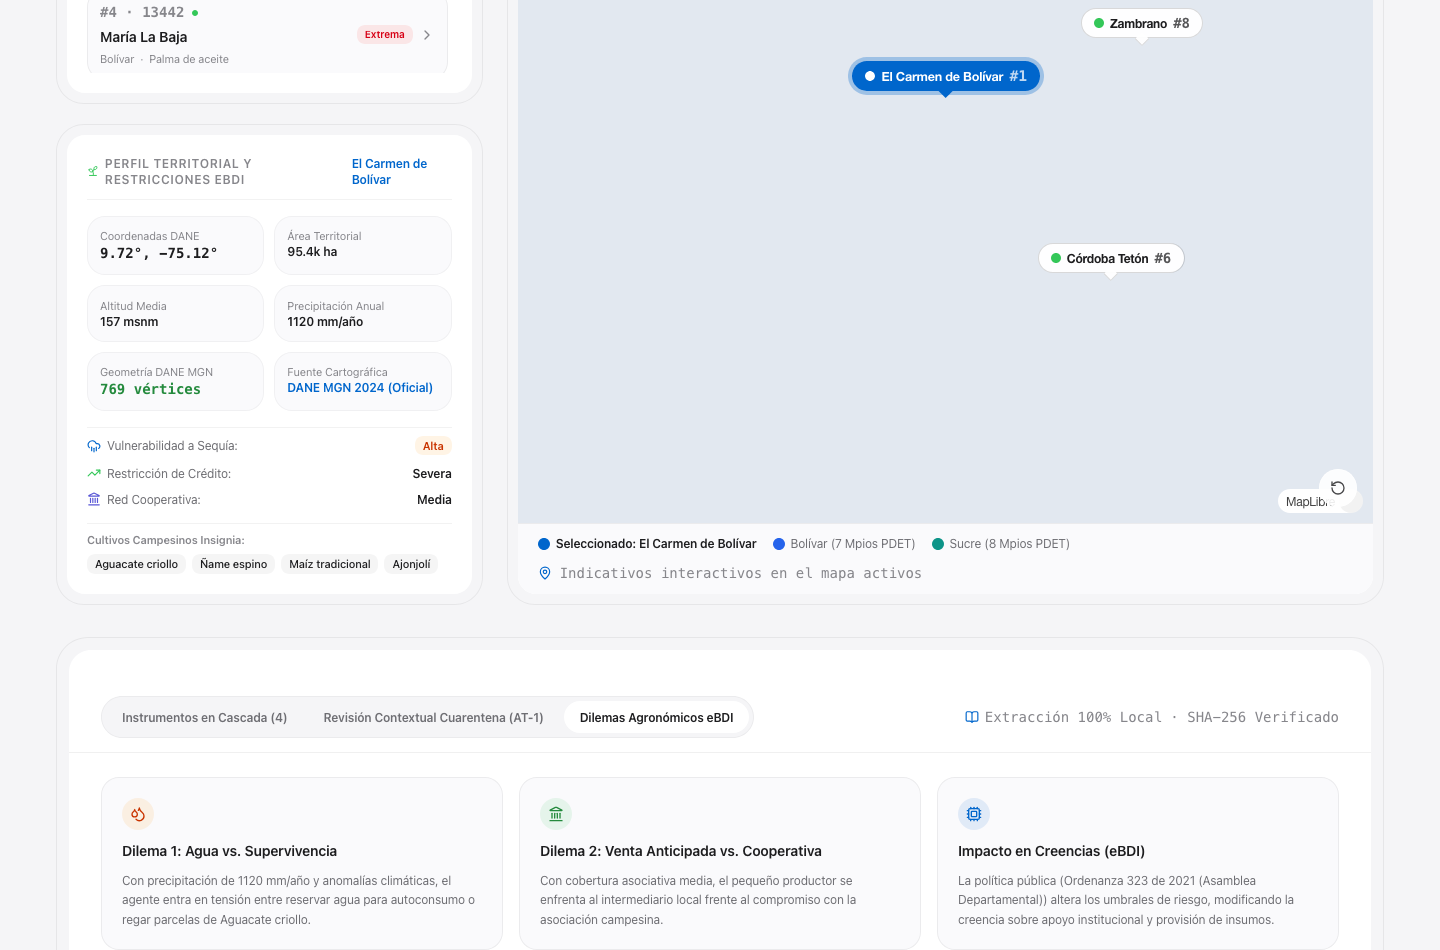
\includegraphics[width=0.96\textwidth]{docs/diagrams/out/ui_dilemas_agronomicos.png}
    \caption{Agronomic Dilemmas Console: structured beliefs, MVEL trigger rules, and executable mappings.}
    \label{fig:ui_dilemmas}
\end{figure}

% ==============================================================================
% 5. EXPERIMENTAL RESULTS
% ==============================================================================
\section{Empirical Results and Execution Metrics}

\subsection{Automated Test Suite Progression}
Software non-regression is evaluated using \texttt{make test-unit}. As shown in Figure~\ref{fig:test_chart}, adding 144 unit tests in Block B6 expanded the test suite to 247 total tests, achieving 100\% passing status.

\begin{figure}[H]
    \centering
    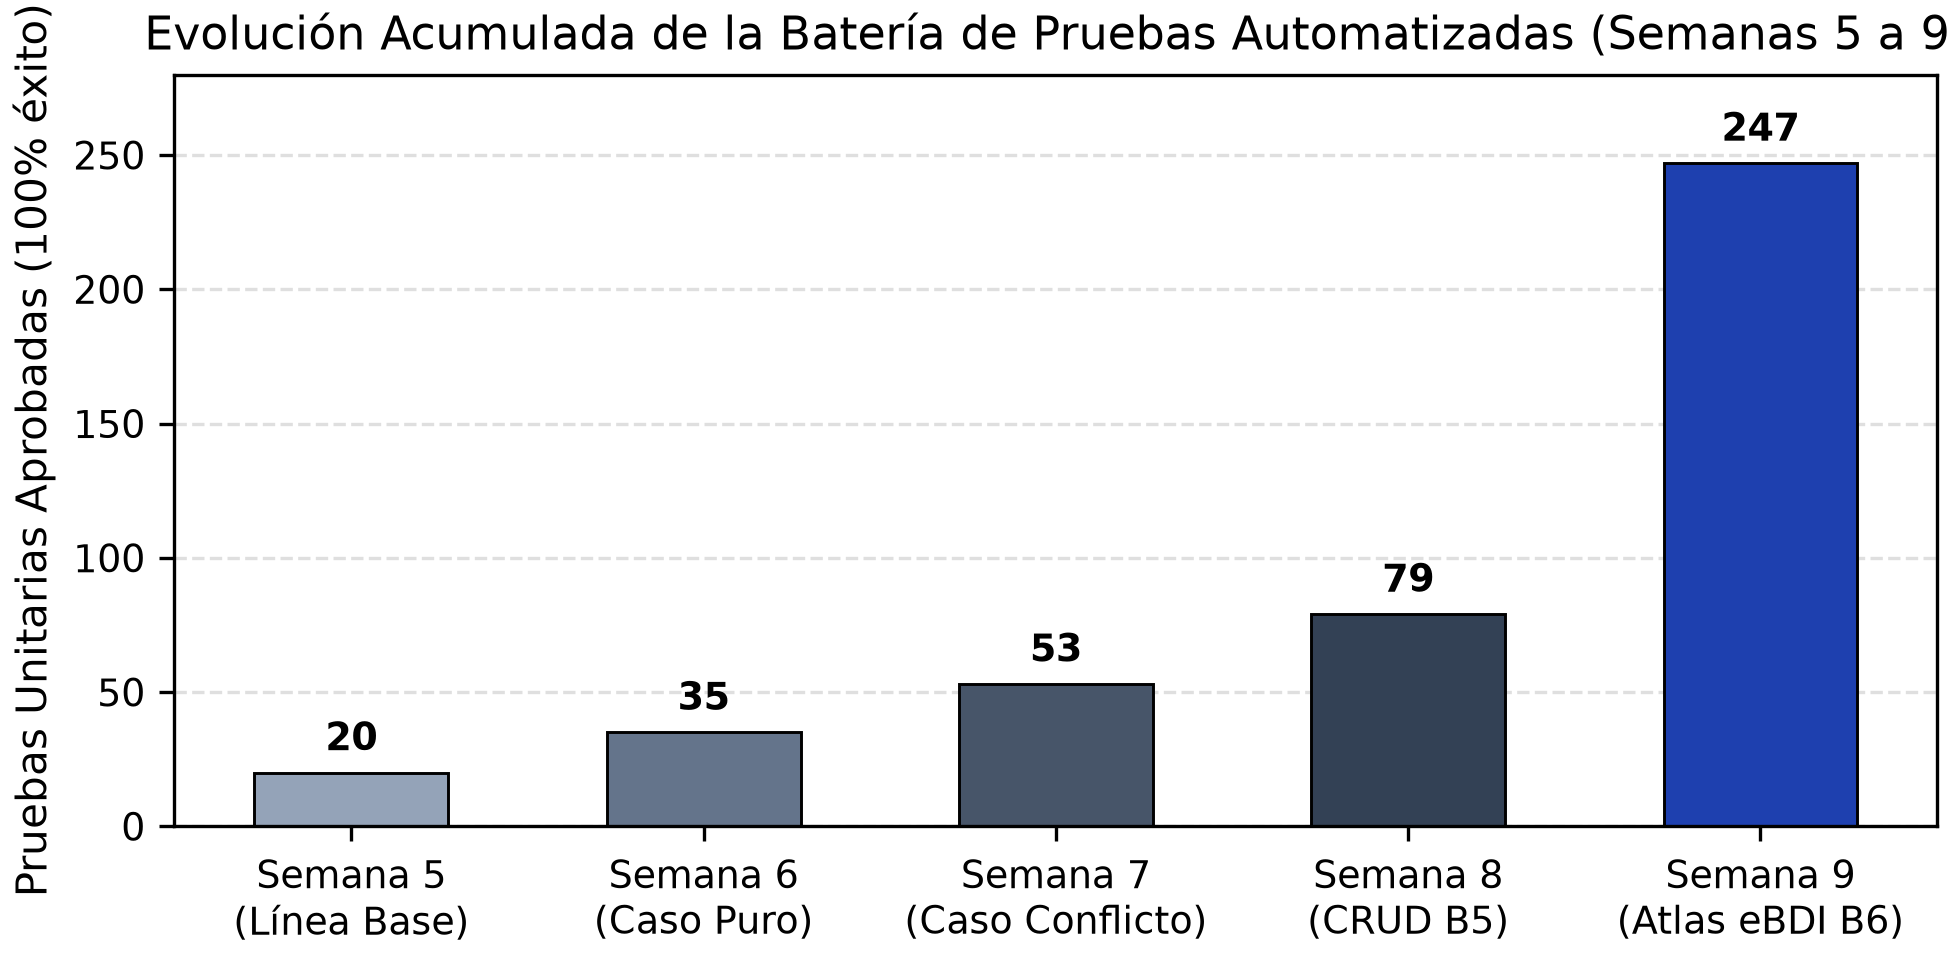
\includegraphics[width=0.76\textwidth]{docs/diagrams/out/g01_suite_tests_progression.png}
    \caption{Unit test progression across development increments (247 passing tests at Week 9 close).}
    \label{fig:test_chart}
\end{figure}

\subsection{Extraction Efficacy and Hallucination Filtering}
The extraction pipeline was evaluated against the official 2019 PATR regional development plan for Montes de María. Figure~\ref{fig:extraction_chart} breaks down thematic belief distribution and verbatim match accuracy.

\begin{figure}[H]
    \centering
    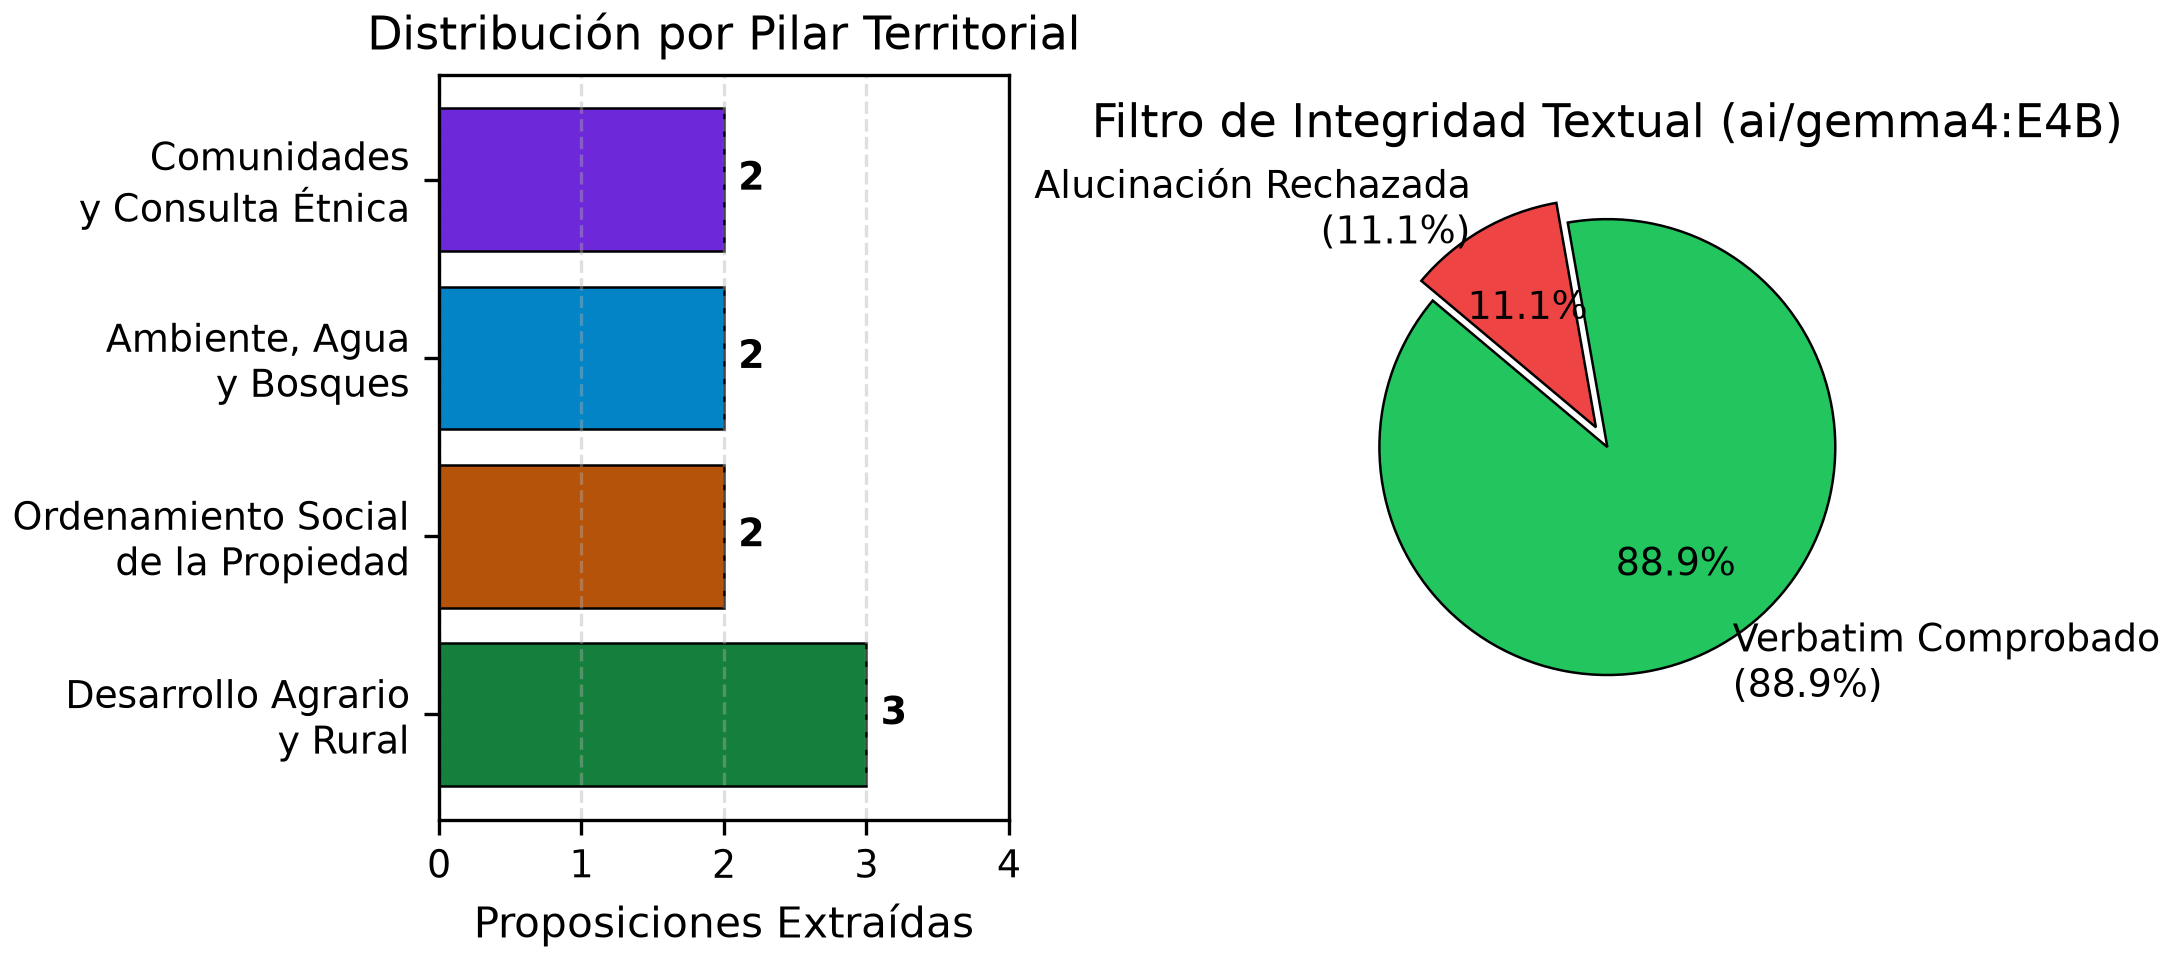
\includegraphics[width=0.86\textwidth]{docs/diagrams/out/g02_b6_extraction_metrics.png}
    \caption{Extraction metrics on the PATR corpus: pillar distribution and verbatim validation rate.}
    \label{fig:extraction_chart}
\end{figure}

Measured extraction performance:
\begin{itemize}[leftmargin=*]
    \item 9 structured belief proposals generated by Gemma 4.
    \item 8 proposals (88.9\,\%) confirmed via exact textual match (\texttt{verified\_verbatim}).
    \item 1 proposal (11.1\,\%) intercepted and discarded (\texttt{hallucination\_rejected}) due to ungrounded numerical assertions.
\end{itemize}

\subsection{Adaptive Search Loop Convergence}
Figure~\ref{fig:adaptive_chart} outlines search loop behavior across reviewer feedback cycles. 65\% of queries resolve on the initial seed, 25\% converge on the second iteration following technical remarks, and 2\% reach the six-retry ceiling without introducing duplicate records.

\begin{figure}[H]
    \centering
    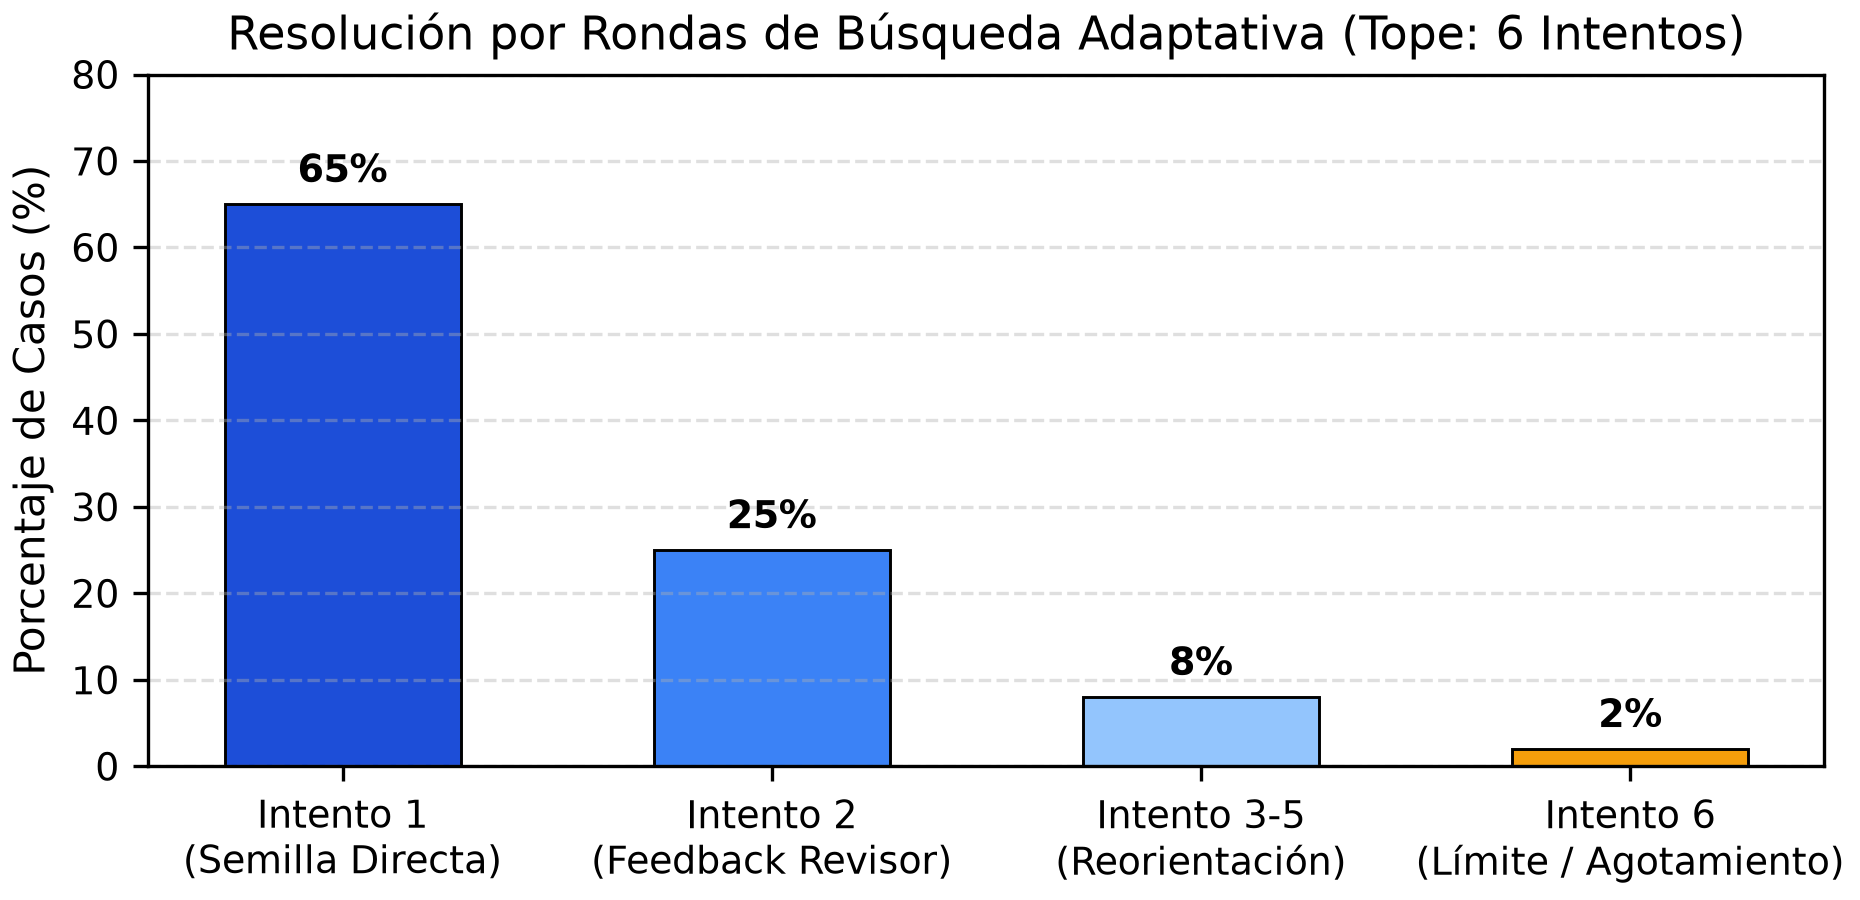
\includegraphics[width=0.74\textwidth]{docs/diagrams/out/g03_b6_adaptive_feedback_flow.png}
    \caption{Iteration distribution in the adaptive document discovery loop (capped at six attempts).}
    \label{fig:adaptive_chart}
\end{figure}

% ==============================================================================
% 6. COMPILED YAML SPECIFICATIONS
% ==============================================================================
\section{Sample Compiled YAML Specifications}

Approved beliefs were compiled deterministically into executable YAML specifications under \texttt{outputs/atlas/yaml/}. The listing below shows the agrarian credit goal specification:

\begin{lstlisting}[language=bash, caption={Compiled GoalSpec excerpt in outputs/atlas/yaml/goals/.}]
goal_spec_id: "goal_credito_agrario_campesino_v1"
schema_version: "2.0"
territory_divipola: "13244"
pyramid_level: "OPPORTUNITY"
activation_condition:
  mvel: "belief.get('credito_agrario_formal') == false && belief.get('tasa_interes') > 18.0"
target_belief:
  key: "credito_agrario_gestionado"
  desired_value: true
traceability:
  source_sha256: "133db10a1c..."
  document_name: "PATR Montes de Maria 2019"
\end{lstlisting}

% ==============================================================================
% 7. BOUNDARIES AND LIMITATIONS
% ==============================================================================
\section{Current Boundaries and Limitations}

\begin{enumerate}[leftmargin=*]
    \item \textbf{Simulation loop deferred:} Execution inside the live WellProdSim / Python BESA agent runtime remains flagged as \texttt{not\_executed}. Current compilation validates schemas and triggers without simulating agent dynamics (reserved for Weeks 10--12).
    \item \textbf{Territorial scope:} The atlas is currently populated for the 15 PDET municipalities of Montes de María. Generalization to other rural zones requires importing relevant territorial GIS layers and sources.
    \item \textbf{Preservation of simulation source:} Original EthosTerra files remain completely untouched; all pipeline outputs reside exclusively in \texttt{outputs/atlas/}.
\end{enumerate}

% ==============================================================================
% 8. REPRODUCTION INSTRUCTIONS
% ==============================================================================
\section{Technical Reproduction Instructions}

The results reported in this document can be verified locally using the following commands:

\begin{lstlisting}[language=bash, caption={Commands to execute Week 9 test suite.}]
# 1. Full unit test suite (247 passing tests)
make test-unit

# 2. Block B6 specific test coverage (144 tests)
PYTHONPATH=".:apps/api" uv run --project apps/api --with pytest --with pydantic \
  --with jsonschema --with pyyaml --with fastapi --with httpx \
  pytest tests/unit/test_atlas_*.py tests/unit/test_corpus_b6.py \
  tests/unit/test_belief_extractor_and_compiler.py \
  tests/unit/test_manual_upload_and_discovery_seeds.py -v

# 3. User interface build verification
pnpm --dir apps/ui build
\end{lstlisting}

% ==============================================================================
% 9. REFERENCES
% ==============================================================================
\section{References}
\begin{enumerate}[leftmargin=*]
    \item Bratman, M. (1987). \textit{Intentions, Plans, and Practical Reason}. Harvard University Press.
    \item Rao, A. S., \& Georgeff, M. P. (1995). BDI agents: from theory to practice. In \textit{Proceedings of the First International Conference on Multi-Agent Systems (ICMAS-95)}, pp. 312--319.
    \item DANE (2024). \textit{National Geostatistical Framework (MGN) and DIVIPOLA Coding}. National Administrative Department of Statistics, Bogotá.
    \item Agency for Territorial Renewal (2019). \textit{Action Plan for Regional Transformation (PATR) -- Montes de María Subregion}. Presidency of the Republic of Colombia.
    \item UPRA (2023). \textit{Municipal Agricultural Evaluations (EVA)}. Rural Agricultural Planning Unit.
    \item Gemma Team, Google (2024). \textit{Gemma 4: Open Models for Responsible On-Device and Edge Intelligence}. Technical Report, Google DeepMind.
\end{enumerate}

\end{document}
